\chapter{Physical Decomposition}\label{phys}

The following sample physical decomposition figures break down the physical components necessary in the primary subsystems. The use of a system engineering approach delves into physical decomposition of the main subsystems at higher detail (namely Environmental Monitoring and Actuation) and are numbered 1 through 2.2 as numbered in the functional decomposition in figure \ref{fig:functional_decomposition}.

\begin{figure}[H]
	\centering
	\fbox{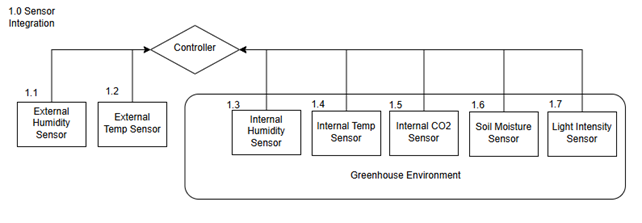
\includegraphics[width=0.8\textwidth]{figs/phys1.png}}
	\caption{Environmental monitoring Physical Decomposition}
	\label{fig:sensor_decomposition}
\end{figure}

\begin{figure}[H]
	\centering
	\fbox{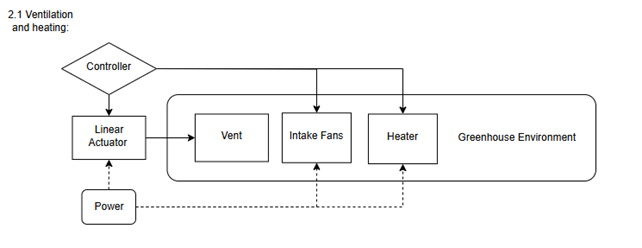
\includegraphics[width=0.8\textwidth]{figs/phys2.png}}
	\caption{Ventilation and Heating Actuation Physical Decomposition}
	\label{fig:ventilation_decomposition}
\end{figure}

\begin{figure}[H]
	\centering
	\fbox{\includegraphics[width=0.8\textwidth]{figs/phys3.png}}
	\caption{Irrigation Physical Decomposition}
	\label{fig:irrigation_decomposition}
\end{figure}


